\documentclass[serif,final]{beamer}
\mode<presentation>{\usetheme{Lankton}}
\usepackage{amsmath,amsfonts,amssymb,pxfonts,xspace}
\usepackage{graphicx}
\graphicspath{{./figures/}}
\usepackage[orientation=landscape,size=a0, scale=1.8]{beamerposter}
\setbeamertemplate{caption}[numbered]

%tikz
\usepackage{tikz}
\usetikzlibrary{shapes,calc,arrows,shadows}
\usepackage{amsmath,bm,times}
\newcommand{\mx}[1]{\mathbf{\bm{#1}}} % Matrix command
\newcommand{\vc}[1]{\mathbf{\bm{#1}}} % Vector command

%-- Header and footer information ----------------------------------
\newcommand{\footleft}{http://www.aalto.fi}
\newcommand{\footright}{narayan.subramaniyam@aalto.fi}
\title{\textit{BrainTrack} : Dynamic identification of brain networks \\ by Bayesian tracking of electrophysiological data}
\author{Narayan Subramaniyam$^{1}$ \quad Filip Tronarp$^{2}$ \quad Simo S\"arkk\"a$^{2}$ \quad Lauri Parkkonen$^{1}$}
\institute{$^{1}$ Department of Neuroscience and Biomedical Engineering \\ $^{2}$ Department of Electrical Engineering and Automation}
%-------------------------------------------------------------------


%-- Main Document --------------------------------------------------
\begin{document}
\begin{frame}{}
  \begin{columns}[t]

    %-- Column 1 ---------------------------------------------------
    \begin{column}{0.45\linewidth}

      %-- Block 1-1
      \begin{block}{Introduction}
      \begin{flushleft}
			\textbf{\color{blue} BrainTrack} is an Academy of Finland -funded project (2015--2019) with the aim to develop a novel method to estimate \textbf{\color{blue}functional brain \\ networks} from magnetoencephalographic (MEG) as well as from scalp and intracranial electroencephalographic (EEG) recordings using \textbf{\color{blue} Bayesian tracking} \cite{sarkka2013bayesian}.
	\end{flushleft}
    \begin{figure}
          \centering
          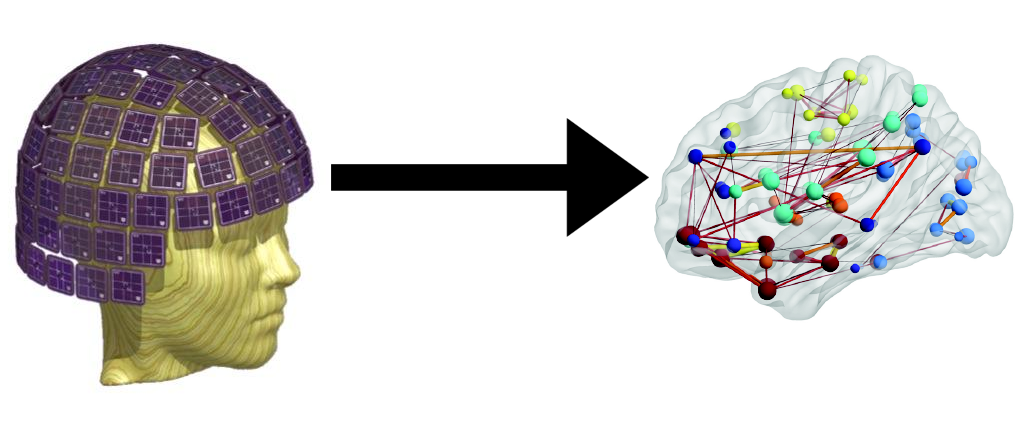
\includegraphics[scale=0.75]{intro_1}
          \caption{Joint estimation of sources and network structure from non-invasive MEG/EEG recordings.}
           \label{fig1}
    \end{figure}
The computational core of BrainTrack is a \textbf{\color{blue} spatio--temporal marginalized particle filter} algorithm \cite{sarkka2013bayesian} that will estimate the network structure along with source parameters. The Bayesian model for the measurements is based on our previous work \cite{sorrentino2009dynamical,chen2013probabilistic}.
    \end{block}

      %-- Block 1-2
    \begin{block}{Significance}
        \begin{enumerate}
		\setlength\itemsep{0.25em}
		\item Tools for better characterization of epileptic activity as a \textbf{\color {blue} dynamic functional network} to aid the accurate 	\textbf{\color {blue} localization} of \textbf{\color {blue} epileptic foci}.
		\item Real-time connectivity estimation for \textbf{\color {blue} neurofeedback} experiments.
		\end{enumerate}
    \end{block}

      %-- Block 1-3
	\begin{block}{International collaboration}
        The project will be done in collaboration with 
        \begin{itemize}
    		    \small
        		\item \textit{Asahikawa Medical University}, Japan (Combined intracranial EEG and MEG recordings)
	        \item \textit{University of Cambridge}, UK (Bayesian methodology)
    		    \item \textit{McGill University}, Canada (Interpretation of connectivity measures and neurofeedback experiments)
    		    \item  \textit{Universit\'e de Montr\'eal}, Canada (Interpretation of connectivity in pathological conditions, intracranial-EEG + MEG recordings )
        \end{itemize}      
    \end{block}
    \end{column}%1

    %-- Column 2 ---------------------------------------------------
    \begin{column}{0.5\linewidth}

      %-- Block 2-1
      \begin{block}{research Framework}     
 	  \begin{figure}
    		    \vspace{2cm}
       		 \centering    
	         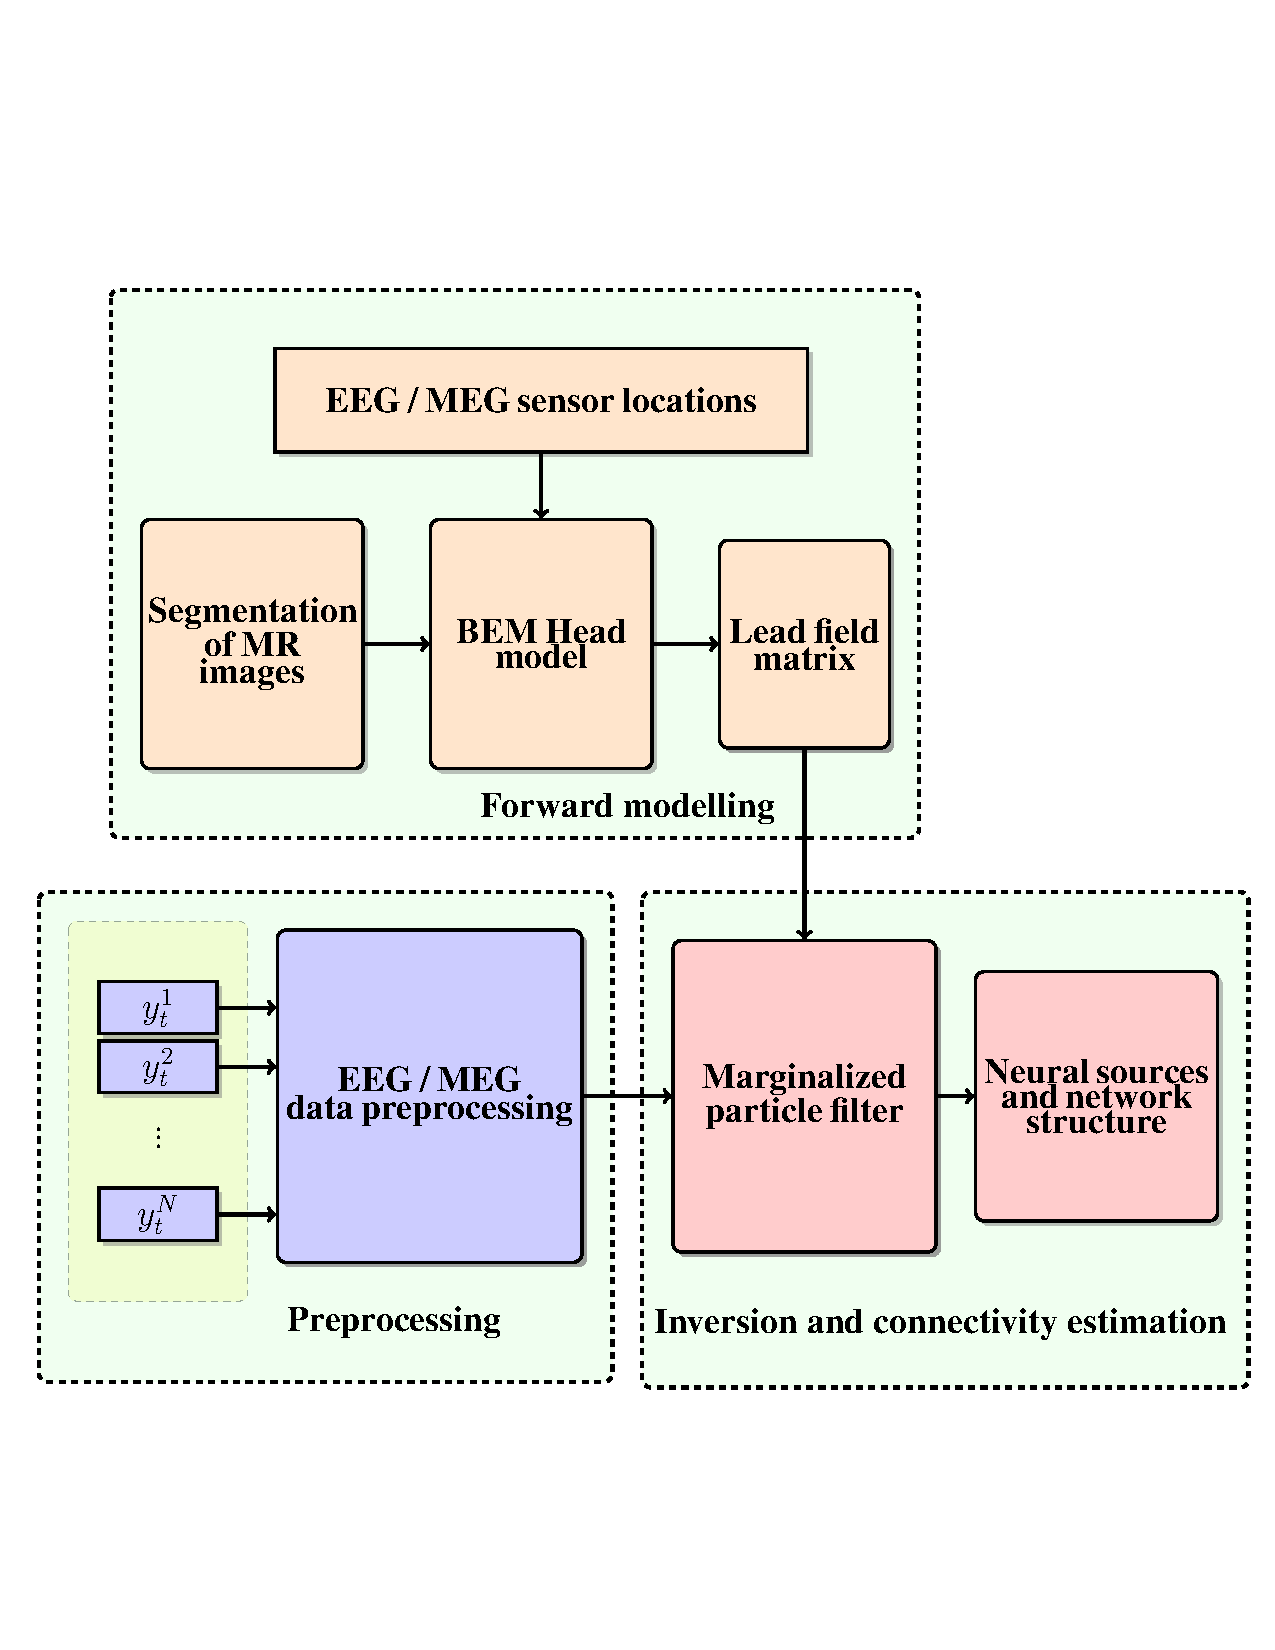
\includegraphics[width = 0.4\linewidth]{framework_ver2}
%         \caption{General framework of the project depicting the workflow}
        \end{figure}
       
    	   \begin{tikzpicture}[remember picture,overlay]
 			 \node[anchor=south west,inner sep=0pt] at ($(current page.south west)+(58cm,38cm)$) {
		     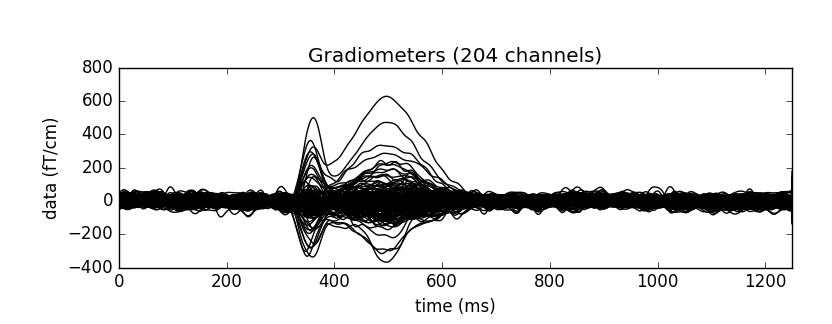
\includegraphics[scale=0.6]{data} };
    	  \end{tikzpicture}

	 \begin{tikzpicture}[remember picture,overlay]
			 \node[anchor=south west,inner sep=0pt] at ($(current page.south west)+(68cm,47cm)$) {
		     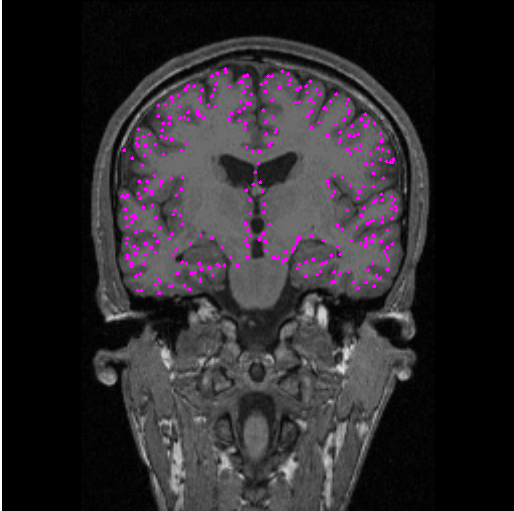
\includegraphics[scale=0.43]{mri} };
	\end{tikzpicture}

	\begin{tikzpicture}[remember picture,overlay]
  			\node[anchor=south west,inner sep=0pt] at ($(current page.south west)+(99cm,37cm)$) {
		     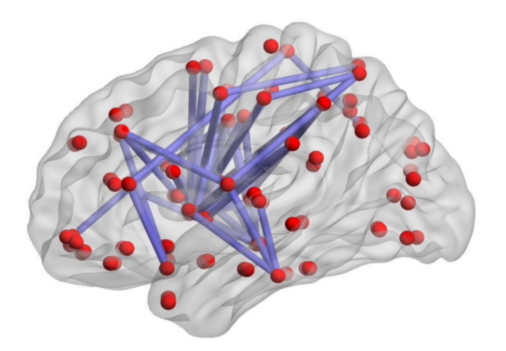
\includegraphics[scale=0.6]{connectivity} };
	\end{tikzpicture}

	\begin{tikzpicture}[remember picture,overlay]
  			\node[anchor=south west,inner sep=0pt] at ($(current page.south west)+(78cm,56cm)$) {
		     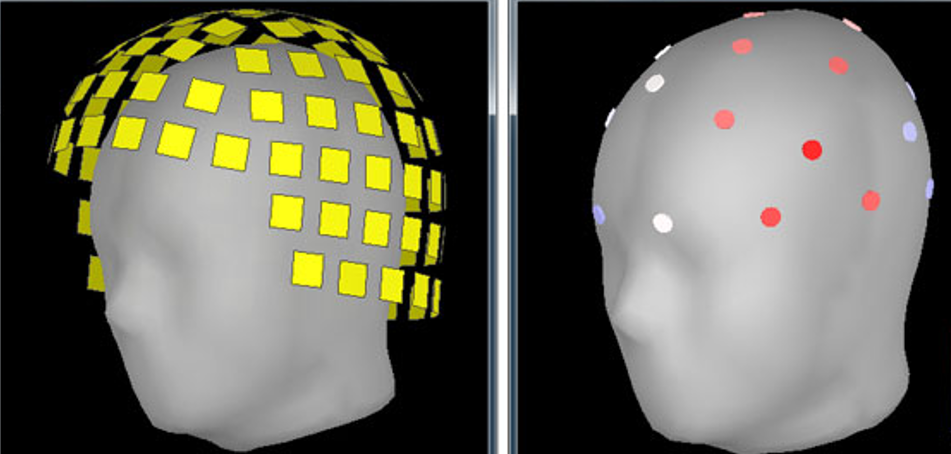
\includegraphics[scale=0.4]{eegmeg} };
	\end{tikzpicture}

	\begin{tikzpicture}[remember picture,overlay]
		  \node[anchor=south west,inner sep=0pt] at ($(current page.south west)+(93.5cm,47cm)$) {
     		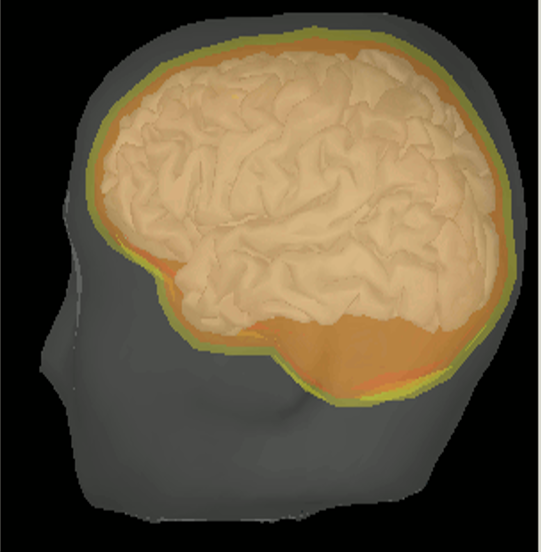
\includegraphics[scale=0.4]{bem} };
	\end{tikzpicture}

	\vspace{-13cm}

    \end{block}

      %-- Block 2-2
      \begin{block}{Expected Results and Impact}
	      \begin{enumerate}
    		  \setlength\itemsep{0.25em}
			\item A platform for \textbf{\color {blue} accurate, real-time} estimation of functional brain connectivity from electrophysiological data. 
			\item Clinical applications: \textbf{\color {blue} Characterization} of spreading pathological brain activity in \textbf{ \color {blue} network disorders} such as epilepsy.
			\item Neuroscience applications: Identification of functional brain networks supporting various \textbf{\color {blue} cognitive functions}.
			\end{enumerate}
      \end{block}
      %-- Block 2-2
      \begin{block}{References}
	      \footnotesize
\bibliographystyle{ieeetr}
\bibliography{refs}
      \end{block}

    \end{column}%2
  \end{columns}
\end{frame}
\end{document}
